\documentclass[11pt]{article}
\usepackage[utf8]{inputenc}

\title{Generative Adversarial Networks}
\author{Jacob Smith}
\date{December 12, 2017}

\usepackage{natbib}
\usepackage{graphicx}

\begin{document}
\maketitle

\begin{abstract}
    General Adversarial Networks have
\end{abstract}

\section{Introduction}
Deep learning have made astounding progress within the past decade. Discriminative models have recently surpassed the abilities of human within the domain of pattern recognition \citep{2014arXiv1404.7828S}. These successes can attributed to vast, high dimension datasets in conjunction with large neural networks using linear activation functions, dropout regularization techniques and backpropagation to update the parameters \citep{2014arXiv1406.2661G}. However, deep learning posses many more ambitious goals. Until recently, success has mostly been seen with supervised classifiers; however, deep generative now competitively rival their discriminative counterpartsdfs.

Generative models learn the joint probability distribution $p(x,y)$ of an input $x$ and label $y$ whereas discriminative models directly learn the conditional probability $p{y|x}$. Knowledge of the probability distribution is created both explicitly and implicitly \citep{Goodfellow-et-al-2016}. Those which do not directly model a probability distribution offer mechanisms which require implicit knowledge of the underlying distribution, such as creating a sample from that distribution \citep{Goodfellow-et-al-2016}. Generative models may be used as classifiers using Bayes rules to calculate $p(x,y)$ \citep{NIPS2001_2020}.

\begin{figure}[h!]
\centering
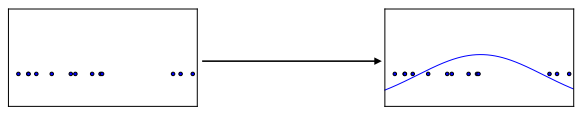
\includegraphics[scale=1.7]{pdf.jpg}
\caption{The process density estimation of one-dimensional data and a Gaussian distribution \citep{2017arXiv170100160G}. Generative models take a dataset $D$, sourced from a distribution $p_data$, a create an estimate of that distribution $p_model$.}
\label{fig:pdf}
\end{figure}

\section{Conclusion}
Generative Adversarial Networks

\bibliographystyle{plain}
\bibliography{references}
\end{document}
